\documentclass[11pt,a4paper]{article}
\usepackage[margin=1in]{geometry}
\usepackage{amsmath,amssymb}
\usepackage{graphicx}
\usepackage{booktabs}
\usepackage{hyperref}
\usepackage{xcolor}
\usepackage{tikz}
\usetikzlibrary{arrows.meta,positioning,shapes.geometric,fit,backgrounds,calc}
\usepackage{listings}
\usepackage{enumitem}
\usepackage{float}
\usepackage{caption}

\lstset{
  basicstyle=\ttfamily\small,
  backgroundcolor=\color{gray!10},
  frame=single,
  breaklines=true,
  columns=fullflexible,
}

\hypersetup{
  colorlinks=true,
  linkcolor=blue!60!black,
  citecolor=blue!60!black,
  urlcolor=blue!60!black,
}

\title{Integrating Temporal Memory into GraphCast:\\Architecture Overview and Alternative Approaches}
\author{Lianghong Mo}
\date{April 2026}

\begin{document}
\maketitle

\begin{abstract}
GraphCast is a state-of-the-art graph neural network for medium-range weather forecasting. It operates autoregressively but lacks explicit temporal memory across prediction steps. This document provides a self-contained overview of the GraphCast architecture, explains how we integrate a Mamba selective state space model to provide cross-rollout memory, presents our experimental findings (the approach does not yet outperform the baseline), and discusses alternative temporal memory mechanisms that may be more effective.
\end{abstract}

\tableofcontents
\newpage

%=============================================================================
\section{GraphCast: Architecture}
%=============================================================================

\subsection{The Weather Prediction Problem}

Numerical weather prediction (NWP) aims to forecast the future atmospheric state given the current and recent observations. The atmosphere is described by a set of physical variables---temperature, wind components, humidity, pressure, geopotential---at discrete grid points across the globe and at multiple pressure levels (altitudes).

Traditional NWP solves partial differential equations (Navier-Stokes, thermodynamics) on a computational grid. GraphCast~\cite{lam2023graphcast} replaces this with a learned mapping: given the atmospheric state at two consecutive time steps ($t{-}\Delta t$ and $t$, where $\Delta t = 6\text{h}$), predict the state at $t{+}\Delta t$.

\subsection{The Encode-Process-Decode Framework}

GraphCast follows an encode-process-decode structure, using an icosahedral mesh as a latent spatial representation:

\begin{figure}[H]
\centering
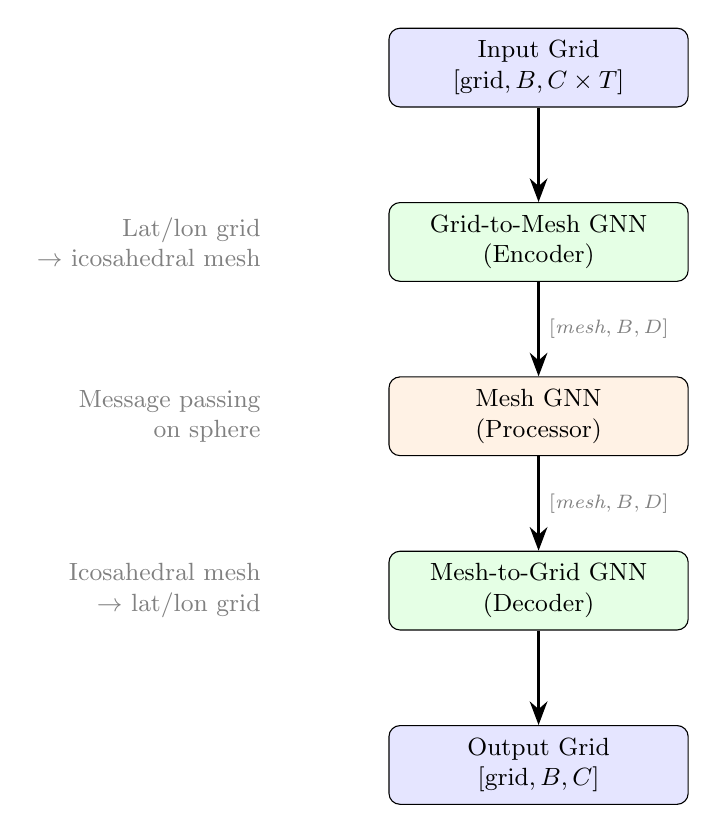
\begin{tikzpicture}[
  box/.style={draw, rounded corners, minimum width=3.8cm, minimum height=1.0cm, align=center, font=\small},
  arrow/.style={-{Stealth[length=3mm]}, thick},
  label/.style={font=\scriptsize\itshape, text=gray},
]

% Nodes
\node[box, fill=blue!10] (input) {Input Grid\\$[\text{grid}, B, C \times T]$};
\node[box, fill=green!10, below=1.2cm of input] (g2m) {Grid-to-Mesh GNN\\(Encoder)};
\node[box, fill=orange!10, below=1.2cm of g2m] (mesh) {Mesh GNN\\(Processor)};
\node[box, fill=green!10, below=1.2cm of mesh] (m2g) {Mesh-to-Grid GNN\\(Decoder)};
\node[box, fill=blue!10, below=1.2cm of m2g] (output) {Output Grid\\$[\text{grid}, B, C]$};

% Arrows
\draw[arrow] (input) -- (g2m);
\draw[arrow] (g2m) -- (mesh) node[midway, right, label] {$[\text{mesh}, B, D]$};
\draw[arrow] (mesh) -- (m2g) node[midway, right, label] {$[\text{mesh}, B, D]$};
\draw[arrow] (m2g) -- (output);

% Side labels
\node[left=1.5cm of g2m, font=\small, text=gray, align=right] {Lat/lon grid\\$\to$ icosahedral mesh};
\node[left=1.5cm of mesh, font=\small, text=gray, align=right] {Message passing\\on sphere};
\node[left=1.5cm of m2g, font=\small, text=gray, align=right] {Icosahedral mesh\\$\to$ lat/lon grid};

\end{tikzpicture}
\caption{GraphCast's encode-process-decode pipeline for a single prediction step.}
\label{fig:graphcast}
\end{figure}

\subsubsection{Step 1: Input Feature Construction}

The input consists of $T$ consecutive atmospheric snapshots (typically $T{=}2$). All time steps are \textbf{concatenated along the channel dimension}:
\[
\mathbf{f}_i = [\mathbf{x}_{t-\Delta t}^{(i)} \;;\; \mathbf{x}_{t}^{(i)}] \in \mathbb{R}^{2C}
\]
where $i$ indexes the $N_\text{grid}$ latitude-longitude grid nodes. This simple concatenation allows a downstream MLP to learn temporal features such as:
\begin{itemize}[nosep]
  \item Velocity: $\mathbf{x}_t - \mathbf{x}_{t-\Delta t}$
  \item Acceleration (with $T{=}4$): $(\mathbf{x}_t - \mathbf{x}_{t-\Delta t}) - (\mathbf{x}_{t-\Delta t} - \mathbf{x}_{t-2\Delta t})$
  \item Any nonlinear combination of the concatenated frames
\end{itemize}

\subsubsection{Step 2: Grid-to-Mesh Encoder}

A graph neural network maps features from the regular lat/lon grid to an \textbf{icosahedral mesh}---a hierarchical triangulation of the sphere. The mesh provides:
\begin{itemize}[nosep]
  \item \textbf{Uniform spatial sampling}: Unlike lat/lon grids (which cluster at the poles), icosahedral meshes have approximately uniform node spacing.
  \item \textbf{Efficient global communication}: At coarse mesh levels, adjacent nodes span large geographic distances, enabling information to propagate globally in few message-passing steps.
\end{itemize}

The encoder performs one message-passing step on a bipartite graph connecting grid nodes to their nearest mesh nodes:
\[
\mathbf{m}_j = \text{GNN}_\text{encode}\left(\{\mathbf{f}_i\}_{i \in \mathcal{N}(j)}\right) \in \mathbb{R}^D
\]
where $j$ indexes mesh nodes and $\mathcal{N}(j)$ are grid nodes within a query radius.

\subsubsection{Step 3: Mesh Processor}

The processor performs $K$ rounds of message passing on the mesh graph (typically $K{=}4$ for the small model, $K{=}16$ for the full model). Each round updates mesh node features based on their mesh neighbors:
\[
\mathbf{m}_j^{(k+1)} = \mathbf{m}_j^{(k)} + \text{MLP}\left(\mathbf{m}_j^{(k)}, \sum_{j' \in \mathcal{N}_\text{mesh}(j)} \text{MLP}([\mathbf{m}_j^{(k)}; \mathbf{m}_{j'}^{(k)}; \mathbf{e}_{jj'}])\right)
\]
This enables global spatial information flow: with $K{=}4$ steps on a mesh with $\sim$2,500 nodes, information can travel from any point on the globe to any other.

\subsubsection{Step 4: Mesh-to-Grid Decoder}

A reverse GNN maps updated mesh features back to the lat/lon grid. The output is a residual prediction:
\[
\hat{\mathbf{x}}_{t+\Delta t} = \mathbf{x}_t + \text{GNN}_\text{decode}(\mathbf{m}^{(K)})
\]

\subsection{Autoregressive Rollout}

For multi-step forecasting, the prediction $\hat{\mathbf{x}}_{t+\Delta t}$ is fed back as input:
\[
(\mathbf{x}_{t-\Delta t}, \mathbf{x}_t) \xrightarrow{\text{predict}} \hat{\mathbf{x}}_{t+\Delta t} \xrightarrow{\text{feed back}} (\mathbf{x}_t, \hat{\mathbf{x}}_{t+\Delta t}) \xrightarrow{\text{predict}} \hat{\mathbf{x}}_{t+2\Delta t} \rightarrow \cdots
\]

\textbf{Critical limitation}: Each step sees only the two most recent frames. There is no mechanism to retain information from earlier steps. The model at step $k$ has no knowledge of the original initial conditions or the intermediate trajectory---it sees only $(\hat{\mathbf{x}}_{t+(k-1)\Delta t}, \hat{\mathbf{x}}_{t+k\Delta t})$.

%=============================================================================
\section{Mamba: Selective State Space Model}
%=============================================================================

\subsection{State Space Models}

State space models (SSMs) are a class of sequence models derived from continuous-time linear systems:
\begin{align}
  \dot{h}(t) &= A h(t) + B x(t) \\
  y(t) &= C h(t) + D x(t)
\end{align}
where $h(t) \in \mathbb{R}^H$ is the hidden state, $x(t)$ is the input, and $y(t)$ is the output. After discretization with step size $\Delta$:
\begin{align}
  h_t &= \bar{A} \, h_{t-1} + \bar{B} \, x_t, \quad \bar{A} = \exp(A \cdot \Delta) \label{eq:ssm_discrete} \\
  y_t &= C \, h_t + D \, x_t
\end{align}

The key property is that $h_t$ is a \textbf{compressed summary of the entire input history} $x_1, x_2, \ldots, x_t$. Unlike Transformers, which require $O(T^2)$ attention over the full sequence, SSMs process sequences in $O(T)$ time with constant memory per step.

\subsection{Mamba's Selective Mechanism}

Standard SSMs use fixed $A, B, C$ matrices. Mamba~\cite{gu2023mamba} makes $B$ and $\Delta$ \textbf{input-dependent}, allowing the model to selectively remember or forget information:
\begin{align}
  \Delta_t &= \text{softplus}(\text{Linear}(x_t)) \quad\text{(data-dependent step size)} \\
  \bar{A}_t &= \exp(A \cdot \Delta_t) \quad\text{(data-dependent decay)} \\
  h_t &= \bar{A}_t \cdot h_{t-1} + (1 - \bar{A}_t) \cdot x_t \label{eq:mamba_state}
\end{align}

When $\Delta_t$ is large, $\bar{A}_t \approx 0$ and the state resets to the current input (``remember this''). When $\Delta_t$ is small, $\bar{A}_t \approx 1$ and the state is preserved (``ignore this input''). This selectivity makes Mamba effective for sequences with variable information density.

\subsection{Our SSM Block}

Each Mamba block in our implementation consists of:

\begin{enumerate}[nosep]
  \item \textbf{Layer normalization} on the input
  \item \textbf{Input projection}: $[\mathbf{u}, \mathbf{g}] = \text{Linear}_{2H}(\mathbf{x}) \in \mathbb{R}^{2H}$
  \item \textbf{Discretization}: $\Delta = \text{softplus}(\text{Linear}_H(\mathbf{u}))$
  \item \textbf{Selective scan} (Eq.~\ref{eq:mamba_state}): $h_t = e^{A \cdot \Delta_t} \cdot h_{t-1} + (1 - e^{A \cdot \Delta_t}) \cdot u_t$
  \item \textbf{Gated output}: $y_t = h_t \odot \sigma(g_t) + s \odot u_t$ \quad (learnable skip $s$)
  \item \textbf{Output projection}: $\text{Linear}_D(y_t)$ back to input dimension
  \item \textbf{Residual connection}: output $= x_t + \text{projected } y_t$
\end{enumerate}

%=============================================================================
\section{Connecting Mamba to GraphCast}
%=============================================================================

\subsection{Where to Insert Temporal Memory}

The natural insertion point is between the encoder and processor, where the atmospheric state is represented as mesh-node features $\mathbf{m} \in \mathbb{R}^{N_\text{mesh} \times B \times D}$. At this point:
\begin{itemize}[nosep]
  \item The features are spatially structured (one vector per mesh node)
  \item The spatial extent is manageable ($\sim$2,500 nodes for mesh\_size=4)
  \item The downstream processor and decoder are unchanged
\end{itemize}

\subsection{Failed Approach: Replace the Encoding Path}

Our first design encoded each input timestep separately through the Grid-to-Mesh GNN, producing a 4D tensor $[\text{time}, \text{mesh}, B, D]$, then applied Mamba over the time axis.

\begin{figure}[H]
\centering
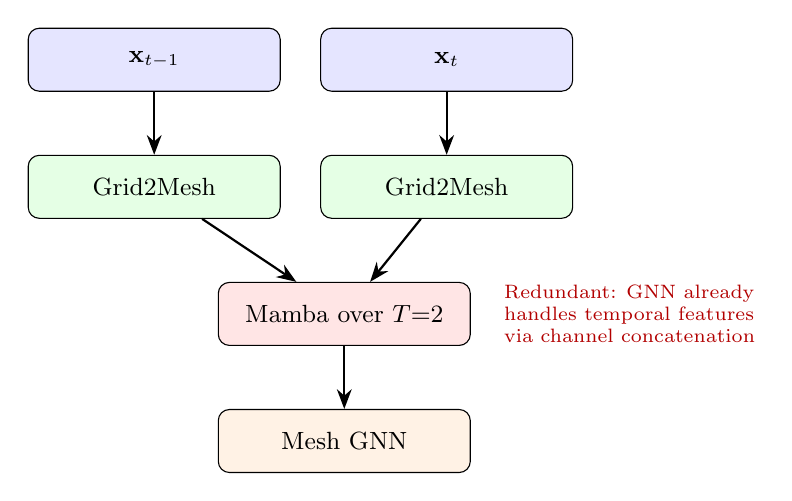
\begin{tikzpicture}[
  box/.style={draw, rounded corners, minimum width=3.2cm, minimum height=0.8cm, align=center, font=\small},
  arrow/.style={-{Stealth[length=2.5mm]}, thick},
  badbox/.style={draw, rounded corners, minimum width=3.2cm, minimum height=0.8cm, align=center, font=\small, fill=red!10},
]

\node[box, fill=blue!10] (in1) {$\mathbf{x}_{t-1}$};
\node[box, fill=blue!10, right=0.5cm of in1] (in2) {$\mathbf{x}_{t}$};
\node[box, fill=green!10, below=0.8cm of in1] (g2m1) {Grid2Mesh};
\node[box, fill=green!10, below=0.8cm of in2] (g2m2) {Grid2Mesh};
\node[badbox, below right=0.8cm and -0.8cm of g2m1] (mamba) {Mamba over $T{=}2$};
\node[box, fill=orange!10, below=0.8cm of mamba] (proc) {Mesh GNN};

\draw[arrow] (in1) -- (g2m1);
\draw[arrow] (in2) -- (g2m2);
\draw[arrow] (g2m1) -- (mamba);
\draw[arrow] (g2m2) -- (mamba);
\draw[arrow] (mamba) -- (proc);

\node[right=0.3cm of mamba, font=\scriptsize, text=red!70!black, align=left] {Redundant: GNN already\\handles temporal features\\via channel concatenation};

\end{tikzpicture}
\caption{Failed approach: per-timestep encoding + Mamba. This changes the encoding path and makes Mamba redundant with the GNN's temporal handling.}
\end{figure}

\textbf{Problems}:
\begin{enumerate}[nosep]
  \item The encoding path differs from baseline (per-frame vs.\ concatenated), confounding comparisons.
  \item Mamba processes only 2--4 frames---information the channel concatenation already captures.
  \item Results: 15--20\% worse than baseline.
\end{enumerate}

\subsection{Current Approach: Residual Memory}

The corrected design preserves the baseline encoding path entirely and injects Mamba as a pure residual:

\begin{figure}[H]
\centering
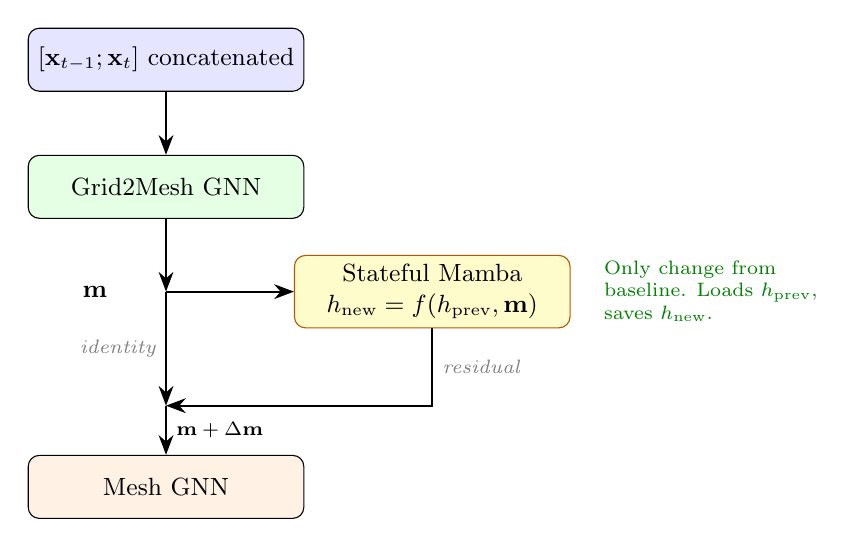
\begin{tikzpicture}[
  box/.style={draw, rounded corners, minimum width=3.5cm, minimum height=0.8cm, align=center, font=\small},
  arrow/.style={-{Stealth[length=2.5mm]}, thick},
  goodbox/.style={draw, rounded corners, minimum width=3.5cm, minimum height=0.8cm, align=center, font=\small, fill=yellow!20, draw=orange!70!black},
]

\node[box, fill=blue!10] (input) {$[\mathbf{x}_{t-1};\mathbf{x}_t]$ concatenated};
\node[box, fill=green!10, below=0.8cm of input] (g2m) {Grid2Mesh GNN};
\node[below=0.8cm of g2m] (split) {};
\node[goodbox, right=1.5cm of split] (mamba) {Stateful Mamba\\$h_\text{new} = f(h_\text{prev}, \mathbf{m})$};
\node[left=0.5cm of split, font=\small] (m) {$\mathbf{m}$};
\node[below=1.2cm of split] (add) {};
\node[box, fill=orange!10, below=0.5cm of add] (proc) {Mesh GNN};

\draw[arrow] (input) -- (g2m);
\draw[arrow] (g2m) -- (split.center);
\draw[arrow] (split.center) -- (mamba);
\draw[arrow] (split.center) -- (add.center) node[midway, left, font=\scriptsize\itshape, text=gray] {identity};
\draw[arrow] (mamba) |- (add.center) node[near start, right, font=\scriptsize\itshape, text=gray] {residual};
\draw[arrow] (add.center) -- (proc) node[midway, right, font=\scriptsize] {$\mathbf{m} + \Delta\mathbf{m}$};

\node[right=0.3cm of mamba, font=\scriptsize, text=green!50!black, align=left] {Only change from\\baseline. Loads $h_\text{prev}$,\\saves $h_\text{new}$.};

\end{tikzpicture}
\caption{Residual memory: identical encoding to baseline, Mamba only injects cross-rollout state as a residual $\Delta\mathbf{m}$.}
\end{figure}

\subsubsection{Cross-Rollout State Threading}

During autoregressive rollout, the Mamba hidden state carries information across prediction steps:

\begin{figure}[H]
\centering
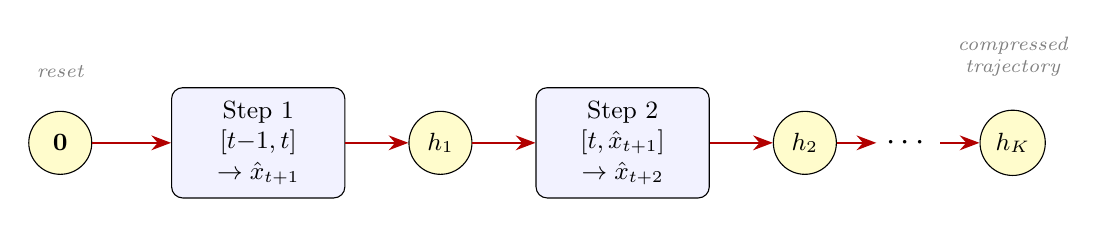
\begin{tikzpicture}[
  rollstep/.style={draw, rounded corners, minimum width=2.2cm, minimum height=1.4cm, align=center, font=\small, fill=blue!5},
  state/.style={draw, circle, minimum size=0.8cm, font=\small\bfseries, fill=yellow!20},
  arrow/.style={-{Stealth[length=2.5mm]}, thick},
  sarrow/.style={-{Stealth[length=2.5mm]}, thick, color=red!70!black},
]

\node[state] (h0) {$\mathbf{0}$};
\node[rollstep, right=1.0cm of h0] (s1) {Step 1\\$[t{-}1, t]$\\$\to \hat{x}_{t+1}$};
\node[state, right=0.8cm of s1] (h1) {$h_1$};
\node[rollstep, right=0.8cm of h1] (s2) {Step 2\\$[t, \hat{x}_{t+1}]$\\$\to \hat{x}_{t+2}$};
\node[state, right=0.8cm of s2] (h2) {$h_2$};
\node[right=0.5cm of h2, font=\large] (dots) {$\cdots$};
\node[state, right=0.5cm of dots] (hk) {$h_K$};

\draw[sarrow] (h0) -- (s1);
\draw[sarrow] (s1) -- (h1);
\draw[sarrow] (h1) -- (s2);
\draw[sarrow] (s2) -- (h2);
\draw[sarrow] (h2) -- (dots);
\draw[sarrow] (dots) -- (hk);

\node[above=0.3cm of h0, font=\scriptsize\itshape, text=gray] {reset};
\node[above=0.3cm of hk, font=\scriptsize\itshape, text=gray, align=center] {compressed\\trajectory};

\end{tikzpicture}
\caption{Hidden state $h_k$ accumulates a compressed summary of the forecast trajectory. The baseline has no equivalent---each step is independent.}
\end{figure}

The three mechanisms enabling this:
\begin{enumerate}[nosep]
  \item \texttt{hk.scan} in GraphCast's autoregressive wrapper threads Haiku state between rollout steps (no code change needed).
  \item \texttt{hk.get\_state}/\texttt{hk.set\_state} in the Mamba block loads the previous hidden state and saves the updated one.
  \item \texttt{\_reset\_ssm\_state()} in the training loop zeros all states before each new training sample, preventing cross-sample leakage.
\end{enumerate}

\subsection{Results So Far}

\begin{table}[H]
\centering
\caption{Residual memory vs.\ baseline (mesh\_size=4, batch=1, input\_steps=2, 6h eval on 2022)}
\begin{tabular}{llccc}
\toprule
Model & target\_steps & RMSE @18k & Baseline @20k & Gap \\
\midrule
Baseline & 2 & --- & 62.41 & --- \\
Residual Memory & 2 & 64.77 & 62.41 & +3.8\% \\
\midrule
Baseline & 4 & --- & 96.08 & --- \\
Residual Memory & 4 & 105.21 & 96.08 & +9.5\% \\
\bottomrule
\end{tabular}
\end{table}

The residual memory architecture does not yet outperform the baseline. The gap is much smaller than our earlier confounded approach ($+3.8\%$ vs.\ $+16\%$), suggesting the encoding path was the primary culprit. However, the Mamba temporal memory itself is not providing enough value to offset its additional parameters and optimization cost.

%=============================================================================
\section{Why Mamba Struggles in This Setting}
%=============================================================================

\begin{enumerate}
  \item \textbf{Information redundancy}: With $T{=}2$ input frames, the model already has access to the current state and its first-order tendency. The residual from Mamba's hidden state adds information from step $k{-}1$, but this is often similar to what the two input frames already encode.

  \item \textbf{Capacity bottleneck}: The hidden state $h \in \mathbb{R}^{128}$ per mesh node must compress the entire atmospheric trajectory. The atmosphere has $\sim$1.4M scalar values per snapshot; $128 \times 2562 \approx 328$K hidden state parameters cannot store a meaningful fraction of the trajectory.

  \item \textbf{Short training rollouts}: With target\_steps=2 or 4, there are only 1--3 state-transfer opportunities. The gradient signal for learning what to store in $h$ is weak.

  \item \textbf{Optimization difficulty}: Gradients must flow through multiple autoregressive steps and the SSM recurrence, creating long credit-assignment chains.
\end{enumerate}

%=============================================================================
\section{Alternative Approaches for Temporal Memory}
%=============================================================================

Given that Mamba has not yet succeeded, what other mechanisms could provide cross-rollout memory?

\subsection{Approach 1: Transformer Cross-Attention over Rollout History}

\textbf{Idea}: At each rollout step $k$, store the mesh latent $\mathbf{m}_k$ in a memory buffer. Use cross-attention to let the current step attend to all previous steps:
\[
\mathbf{m}_k' = \mathbf{m}_k + \text{CrossAttn}(Q{=}\mathbf{m}_k, \; K{=}V{=}[\mathbf{m}_1, \ldots, \mathbf{m}_{k-1}])
\]

\textbf{Pros}:
\begin{itemize}[nosep]
  \item Direct access to all previous states, no information bottleneck
  \item Attention can selectively focus on the most relevant past steps
  \item Well-understood optimization landscape
\end{itemize}

\textbf{Cons}:
\begin{itemize}[nosep]
  \item $O(K \cdot N_\text{mesh})$ memory to store history
  \item $O(K^2)$ attention cost per step (but $K$ is small, e.g.\ 10)
  \item Requires positional encoding for the rollout step index
\end{itemize}

\textbf{Implementation}: Store mesh latents in a buffer that grows during rollout. Apply a small (1--2 layer) cross-attention module after the Grid-to-Mesh encoder.

\subsection{Approach 2: Concatenate Previous Mesh Latent as Extra Input}

\textbf{Idea}: Feed the mesh latent from the \emph{previous rollout step} back as an additional input channel to the current step's mesh processor:
\[
\mathbf{m}_k^\text{input} = [\mathbf{m}_k^\text{encoded} \;;\; \mathbf{m}_{k-1}^\text{processed}]
\]

This is analogous to how GraphCast already uses two atmospheric frames---we simply add a ``previous mesh state'' frame.

\textbf{Pros}:
\begin{itemize}[nosep]
  \item Extremely simple to implement (concatenation + linear projection)
  \item No new module types---uses existing GNN infrastructure
  \item Direct access to previous step's full representation (no bottleneck)
  \item Constant memory overhead (only store one previous step)
\end{itemize}

\textbf{Cons}:
\begin{itemize}[nosep]
  \item Only one step of explicit memory (but this propagates implicitly through the chain)
  \item Doubles the mesh latent input dimension to the processor
\end{itemize}

\textbf{Assessment}: This is arguably the simplest and most promising approach. It mirrors GraphCast's own temporal encoding strategy (channel concatenation) and avoids introducing any new module. The mesh latent is already a compressed, information-rich representation---feeding it back directly may be more effective than compressing it further into a 128-dimensional hidden state.

\subsection{Approach 3: Auxiliary Loss on Temporal Consistency}

\textbf{Idea}: Rather than adding an explicit memory module, add a loss term that encourages temporal consistency in the mesh latent space:
\[
\mathcal{L}_\text{temporal} = \lambda \sum_{k=1}^{K-1} \left\| \frac{\mathbf{m}_{k+1} - \mathbf{m}_k}{\Delta t} - \frac{\mathbf{m}_k - \mathbf{m}_{k-1}}{\Delta t} \right\|^2
\]

This penalizes ``jerky'' changes in the latent trajectory, encouraging smooth evolution and implicitly encoding temporal structure.

\textbf{Pros}:
\begin{itemize}[nosep]
  \item No additional parameters or modules
  \item Regularizes the latent space to be temporally coherent
  \item Easy to implement and tune via $\lambda$
\end{itemize}

\textbf{Cons}:
\begin{itemize}[nosep]
  \item Does not add new information, only constrains representations
  \item May conflict with the primary forecast loss
  \item Requires multi-step rollout during training (target\_steps $> 2$)
\end{itemize}

\subsection{Approach 4: Learned Error Correction Module}

\textbf{Idea}: Train a separate lightweight network that takes the current prediction and an estimate of accumulated error, and outputs a correction:
\[
\hat{\mathbf{x}}_{t+k\Delta t}^\text{corrected} = \hat{\mathbf{x}}_{t+k\Delta t} + \text{CorrectionNet}(\hat{\mathbf{x}}_{t+k\Delta t}, \; k, \; \mathbf{e}_k)
\]
where $\mathbf{e}_k$ is a running estimate of error characteristics (e.g., mean bias, spatial error pattern).

\textbf{Pros}:
\begin{itemize}[nosep]
  \item Directly addresses the error accumulation problem
  \item Can be trained on long rollouts even if the base model is frozen
  \item The correction can be conditioned on the rollout step index $k$
\end{itemize}

\textbf{Cons}:
\begin{itemize}[nosep]
  \item Requires ground truth at each rollout step for training
  \item Two-stage training (base model + correction) adds complexity
  \item May learn to patch over errors rather than prevent them
\end{itemize}

\subsection{Approach 5: Larger Hidden State with Bottleneck Architecture}

\textbf{Idea}: Keep the Mamba approach but address the capacity bottleneck. Use a much larger hidden state ($H{=}1024$ or $2048$) with a bottleneck projection:
\[
\mathbf{m}' = \mathbf{m} + \text{Linear}_{D \leftarrow H}(\text{Mamba}_{H}(\text{Linear}_{H \leftarrow D}(\mathbf{m}), h_\text{prev}))
\]

\textbf{Pros}:
\begin{itemize}[nosep]
  \item Directly addresses the 128-dim capacity bottleneck
  \item Same architecture, just larger
  \item Bottleneck projection keeps the mesh latent dimension unchanged
\end{itemize}

\textbf{Cons}:
\begin{itemize}[nosep]
  \item Significantly more parameters and memory
  \item May still face the optimization difficulties of long-range credit assignment
  \item Does not address the fundamental question of whether temporal memory is useful
\end{itemize}

\subsection{Comparison of Approaches}

\begin{table}[H]
\centering
\caption{Comparison of temporal memory approaches}
\small
\begin{tabular}{p{3.5cm}cccp{3.5cm}}
\toprule
Approach & Complexity & Memory & New Params & Key Advantage \\
\midrule
Mamba residual (current) & Low & $O(N \cdot H)$ & $\sim$130K & Linear-time sequence processing \\
Cross-attention & Medium & $O(K \cdot N \cdot D)$ & $\sim$500K & Direct access to all past states \\
Concat prev.\ latent & Very low & $O(N \cdot D)$ & $\sim$33K & Simplest; mirrors existing design \\
Auxiliary loss & None & None & 0 & No new parameters \\
Error correction & Medium & Low & $\sim$200K & Directly targets error drift \\
Larger Mamba & Low & $O(N \cdot H')$ & $\sim$2M & More expressive state \\
\bottomrule
\end{tabular}
\end{table}

\subsection{Recommended Next Step}

We recommend \textbf{Approach 2: Concatenate Previous Mesh Latent} as the next experiment:
\begin{enumerate}[nosep]
  \item It is the simplest to implement (a few lines of code)
  \item It provides full-resolution memory (no bottleneck)
  \item It mirrors GraphCast's own temporal design principle
  \item If it works, it validates the value of cross-rollout memory; if not, it strongly suggests the problem is elsewhere
\end{enumerate}

The implementation requires only:
\begin{itemize}[nosep]
  \item Storing the mesh latent from the previous rollout step via \texttt{hk.get\_state}/\texttt{hk.set\_state}
  \item Concatenating it with the current mesh latent: $[\mathbf{m}_k; \mathbf{m}_{k-1}] \in \mathbb{R}^{N \times B \times 2D}$
  \item A single linear projection $\text{Linear}_{D \leftarrow 2D}$ to restore the dimension
  \item Zeroing the stored latent at the start of each training sample
\end{itemize}

%=============================================================================
\section{Conclusion}
%=============================================================================

GraphCast's memoryless autoregressive design is a clear architectural limitation for long-range forecasting. We attempted to address this with a Mamba SSM that carries hidden state across rollout steps. After correcting encoding path confounds, the residual memory architecture shows that Mamba does not significantly harm the model (gap reduced from $-$20\% to $-$3.8\%), but it does not help either.

The failure points to a specific bottleneck: compressing an atmospheric trajectory into 128 dimensions is too lossy to be useful. Alternative approaches that avoid this bottleneck---particularly direct latent concatenation (Approach 2) and cross-attention (Approach 1)---may be more effective. The simplest next experiment is to concatenate the previous rollout step's mesh latent as an additional input channel, which provides full-resolution memory with minimal code changes.

\begin{thebibliography}{9}
\bibitem{lam2023graphcast}
R.~Lam et al., ``Learning skillful medium-range global weather forecasting,'' \textit{Science}, vol.~382, no.~6677, pp.~1416--1421, 2023.

\bibitem{gu2023mamba}
A.~Gu and T.~Dao, ``Mamba: Linear-time sequence modeling with selective state spaces,'' \textit{arXiv preprint arXiv:2312.00752}, 2023.
\end{thebibliography}

\end{document}
